\documentclass[12pt,fleqn]{article}\usepackage{../../common}
\begin{document}
Derin Öğrenme ile Go Oyununu Oynamak, DeepMind AlphaGo Zero

Yapay Zeka alanındaki heyecan verici ilerlemelerden biri Google DeepMind
şirketinin AlphaGo programının 17 kez Go şampiyonu olmuş Lee Sedol'u
yenmesiydi. Fakat DeepMind orada durmadı, mimariyi geliştirerek AlphaGo'yu
100-0 yenecek AlphaGo Zero'yu geliştirdi! Yeni mimarinin ilginç tarafı
YZ'nin hiç dış veriye ihtiyaç duymadan eğitilmiş olması. AGZ sıfır
kabiliyet ile başlıyor (clean slate), ve kendisiyle oynaya oynaya Go
şampiyonlarını yenecek hale geliyor.  Bu ve ek ilerlemeleri bu yazıda
paylaşıyoruz.

Mimari

Genel olarak AG ve AGZ'nin benzer bazı özellikleri var. Bunlardan ilki
Monte Carlo Ağaç Aramasının (Monte Carlo Tree Search -MCTS-) bir derin YSA
ile genişletilerek kabiliyetinin ilerletilmiş olması. MCTS konusunu
işledik, herhangi bir tahta pozisyonundan başlayarak simülasyon yapılır, ve
kazanç / kayıp verisi yukarı alınarak karar mekanizması için
kullanılır. Fakat simülasyon yapılırken ve her tahta pozisyonundan hamle
seçenekleri üretilirken ne kadar derine inilecek? Oyun bitene kadar
inilirse bu özellikle Go gibi bir oyunda çok derin ve geniş bir ağaç ortaya
çıkartabilir, bilgisayarlar performans açısından böyle bir ağaçla
zorlanırlar. Çözüm belli bir tahtaya bakarak o oyunun kazanılıp
kazanılmayacağı hakkında ``sezgisel'' bir karar verebilmek. Bu işi örüntü
tanıma üzerinden YSA çok güzel yapabilir. Önceden (kendisiyle oynarken)
elde edilen oyun verisine bakarak, tahta pozisyonları ve o oyunun kazanılıp
kazanılmadığı verisiyle eğitilen ``değer YSA'sı'' artık yeni bir tahtayı
görünce o durumun kazanç şansının olup olmadığını -1,+1 arasında bir değer
ile hesaplayabilir. Bu durumda MCTS'in herhangi bir dalda oyunu sonuna
kadar simüle etmesine gerek yoktur, belli bir seviye sonra durup YSA'ya
kazanç şansını sorar, bu değeri kullanır.

İkinci özellik bir ilke / siyaset / strateji YSA'sı kullanmak, ilke YSA'sı
bir tahtayı girdi olarak alıp, yapılabilecek tüm hamleler için bir kazanç
olasılığı üretebilir, ilke YSA'sin çıktısı potansiyel olarak tüm tahta
hücreleri olabilir [1,3]. MCTS bu çıktıları kazanma olasılığı daha yüksek
olan hamle ağaç dallarını simüle etmek için kullanacaktır.

Yazının geri kalanında 9x9 Go boyutlarını referans alacağız, AG ve AGZ
19x19 oyunu üzerinde işliyor. 

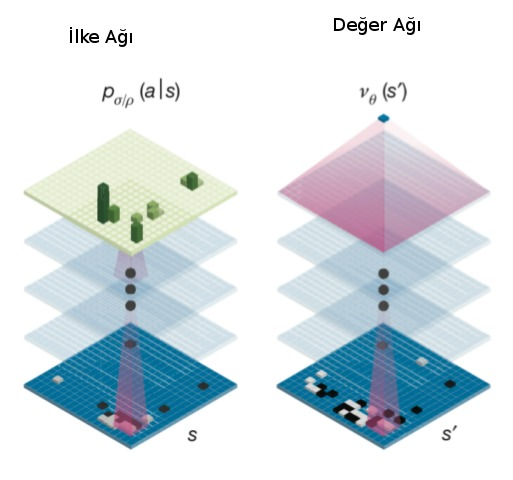
\includegraphics[width=20em]{go_02.jpg}

Bir not düşelim, YSA ``bir tahtayı girdi alıyor'' dedik ama girdi verisi
oldukca zenginleştirilmiş halde, sadece (9,9) boyutunda tek bir tahta
değil, (9,9,17) boyutunda yani 17 katmanlı bir veri ``balyası''. Bu balyayı
hazırlamak için herhangi bir oyun anında tahtaya bakılır, her renk için
(siyah/beyaz) 8 katman yaratılır, bu katmanlardan biri o rengin o andaki
tahtadaki pozisyonu, diğer 7'si hemen önceki 7 adımdaki aynı rengin
pozisyonları, aynı şekilde diğer renk için 8 katman, ve ek bir katman
sıranın kimde olduğu. Tüm bunlar istiflenerek toplam 17 katman
yaratılır. Herhangi bir anda oyunun durumu bu tensor üzerinden
belirtilir. Verinin bu şekilde zenginleştirilmesinin sebebi herhalde
zamansal bağlantıları yakalamaya uğraşmak. 

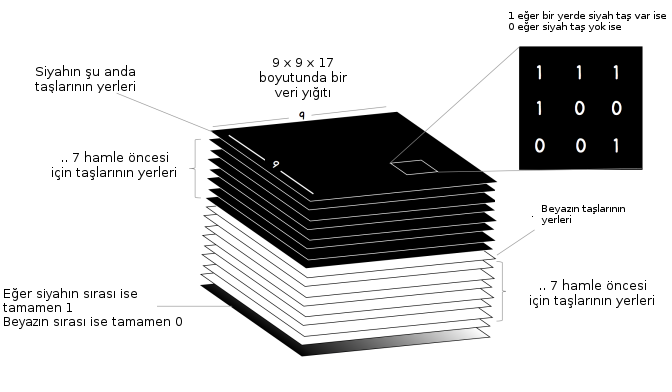
\includegraphics[width=30em]{go_01.png}

AlphaGo Zero

AGZ'nin yaptığı ilerlemeler ise şunlar [3]: AlphaGo değer ve ilke için iki
ayrı ağ kullanıyordu. AGZ'de değer ve ilke YZ'leri birleştirilerek tek bir
YSA ile iki çıktı üretilmesi sağlanıyor, bu yapıya esprili bir şekilde
``iki başlı canavar (two-headed monster)'' ismi de veriliyor. Bu mimari
biraz garip gelebilir, çünkü çoğu uygulamada genellikle tek bir çıktı
kullanılır, mesela bir resimde kedi olup olmadığını tahmin edecek bir YZ
tek bir ikisel çıktı ile bunu yapabilir, ya da resmin belli kategorilere
ait olup olmadığı tek bir vektör çıktısı ile, bu vektörde obje olasılıkları
vardır. Fakat biraz düşününce iki farklı çıktılı yapının niye işlediğini
anlayabiliriz, sonuçta YZ bir fonksiyonu yaklaşık olarak temsil etmeye
çabalar, eğitim sırasında kafa \#1 fonksiyonu bir tahmin üretir, ve eğitim
o kafanın yaptığı tahmine sonuç veren parametreleri günceller, aynı şekilde
kafa \#2 için düzeltme yapılır.

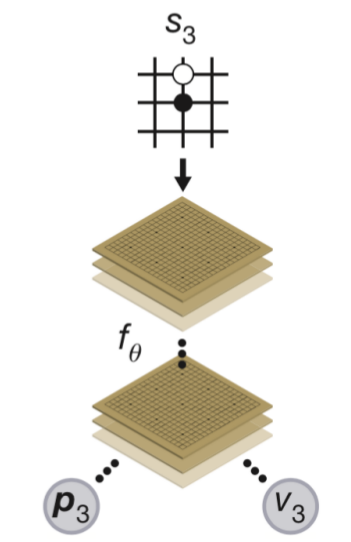
\includegraphics[width=15em]{go_03.png}

İkinci bir AGZ ilerlemesi artıksal ağ (residual network) adı verilen bir
derin YSA yapısı kullanmak. Artıksal ağlar pür evrişimsel ağların daha
gelişmiş hali, bu yapılarda evrişimsel ağda bölge atlaması yapılarak
sonraki bölgelere direk / kısayol bağlantıları koyuluyor [6]. Örnek bir
yapı altta,

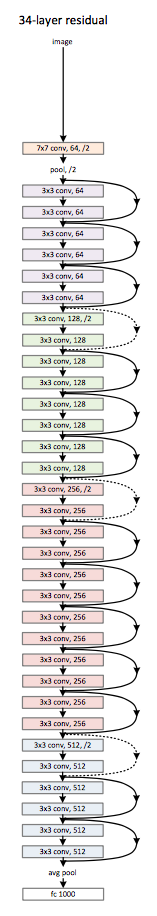
\includegraphics[width=10em]{resnet34.png}

Üçüncü ilerleme ise AGZ'nin kendisine karşı oynayarak kendini eğitmesi (AG
için başkaların oynadığı oyunların kayıtları kullanıldı). DeepMind
bilimcileri araştırmaları sırasında şunu anladılar: hangi baz mimariyle
başlarsak başlayalım, MCTS onu daha iyileştirir. Bu durumda herhangi bir YZ
alınır ki başta ağırlık değerleri rasgele yani hiç bir doğru karar vermez,
ama bu YZ, MCTS ile daha iyi performans gösterecektir, bu sırada oyundan
eğitim verisi toplanır ve bu veri YZ'yi iyileştirmek için ağa uygulanır, ve
işlem başa dönerek devam edilir. Bu sayede en kötü performanstan en iyisine
doğru ilerlemek mümkündür.

Eğitim verisinde hedefin ne olduğunu daha iyi vurgulamak gerekirse, değer
kafası için bu tek bir değer, ilke kafası için tüm 9x9 tahta
pozisyonlarında hangi hamlenin yapılmış olduğu, o hücre 1 diğerleri 0
değerinde olacak. Bu şekilde eğitilen YSA, ilke tahmini üreteceği zaman tüm
hücrelerde olasılık değerleri üretecektir.

Alttaki kod [4]'u baz almıştır. Eğitmek için \verb!train.py! kullanılır,
eğitim sırasında en son YSA belli aralıklarla sürekli kaydedilecektir,
eğitim sonunda ya da yeterince eğitilince işlem durulabilir, ve
\verb!gnugo_play.py! kaydedilen aynı modeli kullanarak GnuGo [1] programına
karşı oynatılabilir. YSA olarak biz ResNet yerine daha basit bir yapı
kullandık,

\begin{minted}[fontsize=\footnotesize]{python}
import simplenet
simplenet.PolicyValue.create_network()
\end{minted}

\begin{verbatim}
Tensor("input_1:0", shape=(?, 17, 9, 9), dtype=float32)
Tensor("conv2d/BiasAdd:0", shape=(?, 17, 9, 64), dtype=float32)
Tensor("batch_normalization/batchnorm/add_1:0", shape=(?, 17, 9, 64), dtype=float32)
Tensor("conv2d_2/BiasAdd:0", shape=(?, 17, 9, 128), dtype=float32)
Tensor("batch_normalization_2/batchnorm/add_1:0", shape=(?, 17, 9, 128), dtype=float32)
------------- value -------------------
Tensor("conv2d_3/BiasAdd:0", shape=(?, 17, 9, 2), dtype=float32)
Tensor("activation_3/Relu:0", shape=(?, 17, 9, 2), dtype=float32)
Tensor("flatten/Reshape:0", shape=(?, 306), dtype=float32)
policy_output Tensor("activation_4/Softmax:0", shape=(?, 82), dtype=float32)
------------- policy -------------------
Tensor("conv2d_4/BiasAdd:0", shape=(?, 17, 9, 1), dtype=float32)
Tensor("activation_5/Relu:0", shape=(?, 17, 9, 1), dtype=float32)
Tensor("flatten_2/Reshape:0", shape=(?, 153), dtype=float32)
Tensor("dense_2/BiasAdd:0", shape=(?, 256), dtype=float32)
Tensor("activation_6/Relu:0", shape=(?, 256), dtype=float32)
Tensor("dense_3/BiasAdd:0", shape=(?, 1), dtype=float32)
Tensor("dense_3/BiasAdd:0", shape=(?, 1), dtype=float32)
Out[1]: <tensorflow.python.keras._impl.keras.engine.training.Model at 0x7fa2dd30de50>
\end{verbatim}

\inputminted[fontsize=\footnotesize]{python}{mcts.py}

\inputminted[fontsize=\footnotesize]{python}{train.py}

\inputminted[fontsize=\footnotesize]{python}{simplenet.py}

İki YSA kendisine karşı oynarken aynı ağırlıklara sahip iki farklı YSA ile
başlıyoruz, ve oyun sonuçlarını kullanarak sadece birini
güncelliyoruz. Eğer her toptan demeti (minibatch) ile her iki YSA'yı
güncelleseydik birbirlerinden farklılaşmaları zorlaşabilirdi. Ama döngünün
daha ileri bir noktasında esitleme yapariz yine de, ilk YSA'yı
güncellenenin ağırlıklarını diskten okuyarak güncelliyoruz, ve böyle devam
ediyor. AGZ tasarımcıları ``en iyi'' olan ağırlıklara geçmeden yeni YSA'nın
diğerini yüzde 55'ten fazla yenmesi şartını koymuşlar, tam donanımla
testleri yapanlar bunu takip ederse iyi olur.

Üstteki mimari birkaç saat eğitim sonrası GnuGo (kendi YZ'si olan bir dış
Go programı) başlangıç, orta seviyelerini yenebiliyor. Okuyucular, grafik
kartlı güçlü bir mimaride, ya üstteki YSA'yı derinleştirerek (daha fazla
evrişim filtresi ekleyerek), ya da \verb!resnet.py! ile, ve \verb!n_play!'i
arttırarak daha fazla simülasyonla sonuçları daha da iyileştirmeye
uğraşabilirler.

Kaynaklar

[1] Bayramlı, 
    {\em Go Oyunu, GnuGo}, 
    \url{https://burakbayramli.github.io/dersblog/sk/2018/02/go-gnugo.html}

[2] Silver, {\em Mastering the game of Go with deep neural networks and tree search}, \url{https://www.nature.com/articles/nature16961}

[3] Weidman, {\em The 3 Tricks That Made AlphaGo Zero Work}, \url{https://hackernoon.com/the-3-tricks-that-made-alphago-zero-work-f3d47b6686ef}

[4] Yi, {\em A reproduction of Alphago Zero in 'Mastering the game of Go without human knowledge'}, \url{https://github.com/sangyi92/alphago_zero}

[5] {\em AlphaGo Zero Cheat Sheet}, \url{https://applied-data.science/static/main/res/alpha_go_zero_cheat_sheet.png}

[6] Kristiadi, {\em Residual Net}, \url{https://wiseodd.github.io/techblog/2016/10/13/residual-net/}



\end{document}
